\section{Promptable and Grounded Segmentation}
\label{sec:promptable-grounded-segmentation}

The previous section reviewed open-vocabulary segmentation as the transfer of text-defined categories to pixels, regions, and masks. This section studies the second main technical route: promptable and grounded segmentation. Its central objective is different from pure open-vocabulary recognition. Instead of asking only whether a model can assign an unseen class name to a dense region, it asks how a user, a phrase, a visual cue, or a generated response can control which region should be segmented and how that region should be linked back to language. This route therefore sits between open-vocabulary segmentation and reasoning segmentation. It inherits mask priors from promptable segmenters, semantic flexibility from VLMs, and language-region supervision from referring and grounding tasks.

Existing work can be broadly grouped into five routes, as summarized in Table~\ref{tab:promptable-grounded-methods}. The first route treats SAM and SAM2 as reusable class-agnostic mask priors. The second route composes open-set detectors, grounding models, and SAM-like mask decoders into Grounded-SAM pipelines. The third route learns region-word or mask-text alignment directly for referring expression segmentation and grounded conversation. The fourth route adapts foundation models with prompts, visual references, position cues, or lightweight projectors. The fifth route builds pixel-grounded multimodal interfaces, where a model can converse, point, ground, and segment through the same language interface. These routes are not mutually exclusive. Their differences mainly lie in where language enters the system: before mask generation, during mask decoding, after proposal generation, or inside an MLLM response.

\begin{table*}[t]
\centering
\small
\setlength{\tabcolsep}{5pt}
\renewcommand{\arraystretch}{1.34}
\caption{Representative promptable and grounded segmentation methods. The table follows the same indexing function as Table~\ref{tab:open-vocab-methods}: it records the route, foundation prior, prompt or grounding interface, and the main contribution or limitation rather than serving as a leaderboard.}
\label{tab:promptable-grounded-methods}
\begin{tabularx}{\textwidth}{>{\raggedright\arraybackslash}p{0.16\textwidth}>{\raggedright\arraybackslash}X>{\raggedright\arraybackslash}p{0.16\textwidth}>{\raggedright\arraybackslash}p{0.20\textwidth}>{\raggedright\arraybackslash}p{0.23\textwidth}}
\toprule
Route & Representative methods & Foundation or prior & Prompt or grounding interface & Main contribution and typical limitation \\
\midrule
Class-agnostic promptable mask prior & SAM~\citep{kirillov2023sam}; SAM2~\citep{ravi2024sam2}; FocSAM~\citep{huangFocsamDelvingDeeply2024}; Inter2Former~\citep{huangInter2FormerDynamicHybrid2025} & Promptable mask encoder-decoder, streaming memory for video, efficient interactive segmentation modules & Points, boxes, masks, clicks, or video prompts & Provides strong reusable spatial priors and interactive masks; semantics must be supplied by detectors, VLMs, MLLMs, or task-specific adaptation. \\
SAM/SAM2 for open-vocabulary segmentation & Sambor~\citep{xhanBoostingSegmentAnything2025}; ESC-Net~\citep{mleeEffectiveSAMCombination2025}; OpenWorldSAM~\citep{sgxiaoOpenworldsamExtendingSam22026}; X-SAM~\citep{hwangXSAMSegmentAnything2026} & SAM or SAM2 with open-set detectors, VLM embeddings, MLLM interfaces, or promptable decoders & Category names, referring expressions, sentence-level prompts, or visual grounded prompts & Extends promptable masks toward language-defined categories and unified segmentation; performance depends on semantic injection, instance disambiguation, and proposal-mask calibration. \\
Grounded-SAM composition & Grounding DINO~\citep{liu2024groundingdino} with SAM~\citep{kirillov2023sam} and SAM2~\citep{ravi2024sam2}; TGS-Agent~\citep{zhouThinkYouSegment2026}; AL-Ref-SAM2~\citep{huangUnleashingTemporalspatialReasoning2025}; SAMWise~\citep{cuttanoSamwiseInfusingWisdom2025} & Open-set detector or grounding model plus SAM/SAM2 mask generator & Text query first localizes boxes or candidate objects, then SAM/SAM2 produces masks & Decouples text localization from precise segmentation and works well in training-free or weakly supervised settings; errors propagate from detector boxes, frame selection, and prompt quality. \\
Referring and mask-text alignment & Prompt-RIS~\citep{cshangPromptdrivenReferringImage2024}; curriculum point prompting~\citep{daiCurriculumPointPrompting2024}; Mask Grounding~\citep{chngMaskGroundingReferring2024}; OneRef~\citep{xiaoOnerefUnifiedOnetower2024}; RAS~\citep{caoReferAnySegmentation2025} & CLIP/SAM composition, one-tower vision-language transformers, mask visual-language modeling & Referring expressions, primary words, point prompts, mask groups, visual-language prompts & Learns fine-grained phrase-mask or token-mask correspondence beyond flat category labels; complex relations, absent targets, and multiple valid masks remain difficult. \\
Pixel-grounded multimodal interfaces & Kosmos-2~\citep{pengGroundingMultimodalLarge2024}; Ferret~\citep{youFerretReferGround2024}; Osprey~\citep{yuanOspreyPixelUnderstanding2024}; PixelLM~\citep{xuPixelalignedLanguageModel2024}; LLaVA-Grounding~\citep{zhangLlavagroundingGroundedVisual2024}; GLaMM~\citep{rasheedGlammPixelGrounding2024}; GroundingSuite~\citep{huGroundingSuiteMeasuringComplex2025} & MLLMs with coordinates, region features, mask-aware extractors, or grounded conversation data & Boxes, points, free-form regions, location tokens, mask-text instructions, grounded responses & Turns grounding into a language interface and supports region description, dense word grounding, and grounded chat; mask faithfulness and hallucination control require explicit evaluation. \\
Prompt and projector adaptation & Show-or-Tell~\citep{grosiShowTellBenchmark2025}; visual position prompts~\citep{tangVisualPositionPrompt2026}; SAM visual projectors~\citep{yangRepurposingSAMEfficient2026}; zero-shot RIS feature refinement~\citep{wangIterprimeZeroshotReferring2025} & CLIP, SAM, MLLMs, visual reference prompts, position-aware prompts & Text prompts, visual references, spatial prompts, semantic superpixels, visual words & Studies how prompt modality and efficient projection affect grounding; comparisons must control prompt source, prompt count, token budget, and target-domain usage. \\
\bottomrule
\end{tabularx}
\end{table*}

\subsection{SAM and SAM2 as mask priors}

Promptable segmentation changes the segmentation interface from category prediction to mask generation under user control. SAM introduced a foundation-model formulation in which an image encoder, prompt encoder, and lightweight mask decoder produce masks from sparse or dense prompts such as points, boxes, and masks~\citep{kirillov2023sam}. SAM2 extends this idea to images and videos through a streaming-memory architecture and a data engine for interactive video mask collection~\citep{ravi2024sam2}. In the context of this survey, the important contribution of SAM-style models is not open-vocabulary semantics by themselves. Their contribution is a reusable spatial prior: a model can often produce accurate class-agnostic masks once a target location or prompt is specified.

\begin{figure*}[htbp]
    \centering
    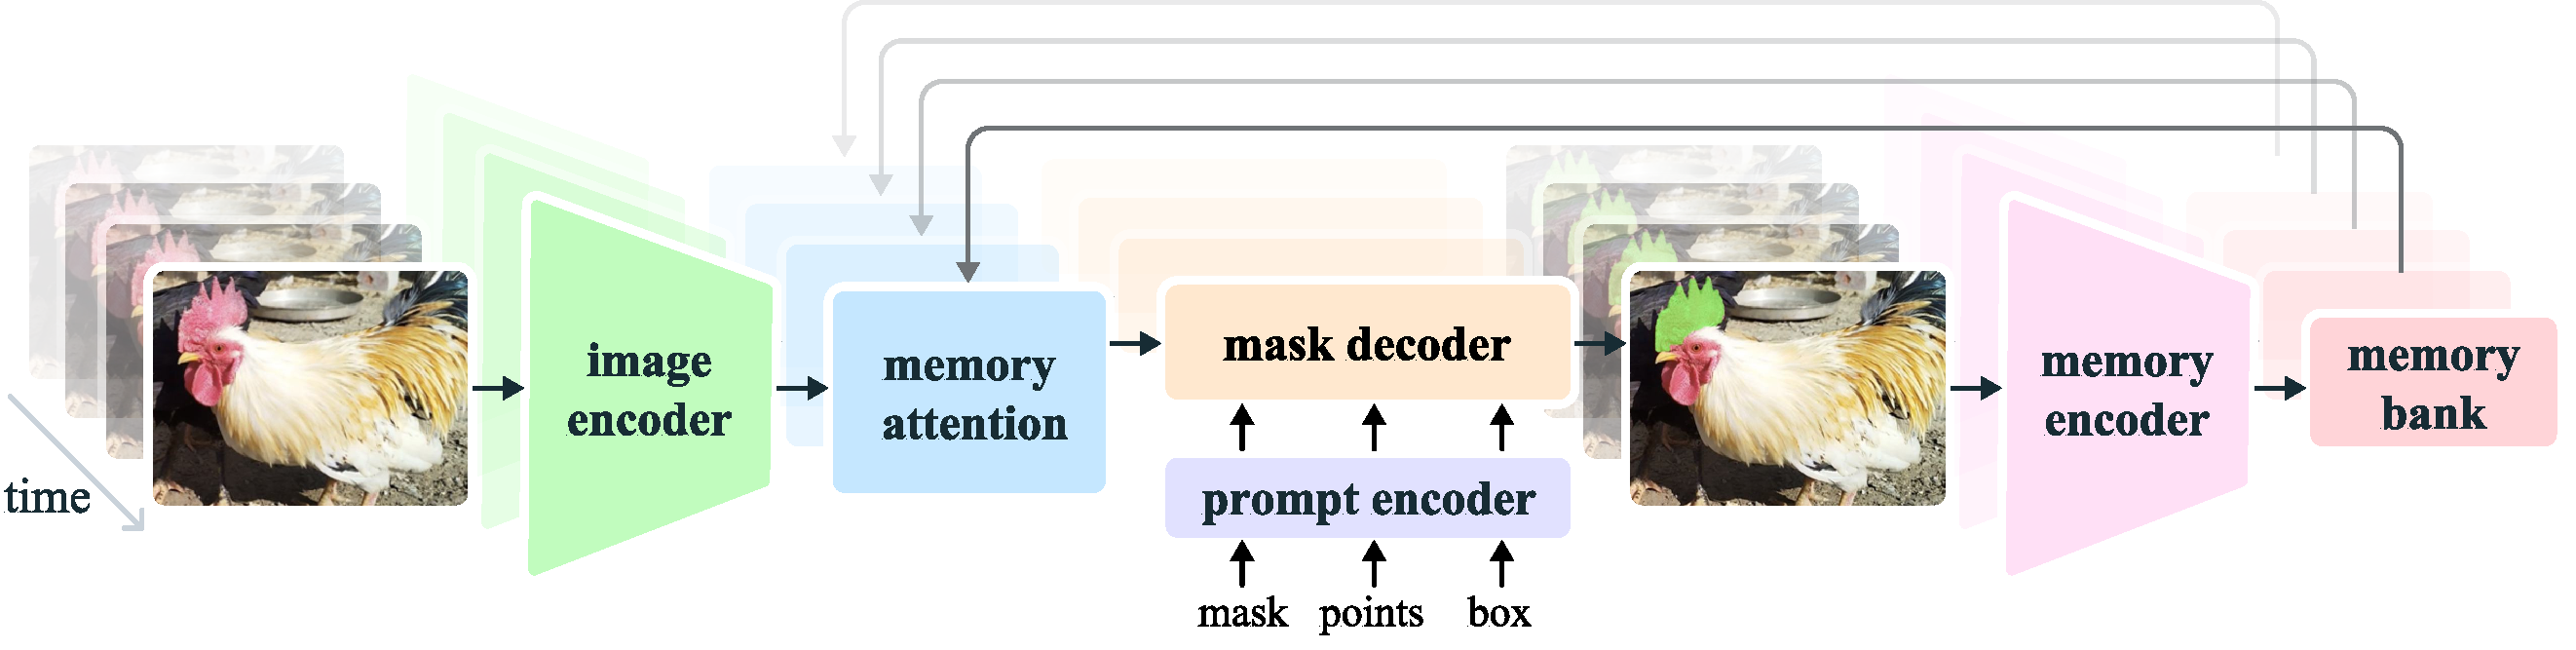
\includegraphics[width=0.98\textwidth]{Fig/fig_SAM2.pdf}
    \caption{SAM2 as a promptable mask prior for images and videos. A frame is encoded by the image encoder, combined with previous-frame memories through memory attention, and decoded with user prompts such as masks, points, or boxes. The predicted mask is then encoded into a memory bank, enabling later frames to reuse temporal information for interactive video segmentation~\citep{ravi2024sam2}.}
    \label{fig:promptable-sam2}
\end{figure*}


Fig.~\ref{fig:promptable-sam2} shows why SAM2 is especially important for the later video and grounded settings: prompts are not processed in isolation, but interact with a memory bank that carries object information across time. This mask-prior view explains why many later methods use SAM as a component rather than a complete solution. FocSAM revisits the interactive pipeline and argues that SAM's fixed image preprocessing and lightweight decoder can be unstable for difficult samples; it introduces target-focused attention and dynamic activation to improve interactive segmentation efficiency~\citep{huangFocsamDelvingDeeply2024}. Inter2Former studies the efficiency side of interactive segmentation by allocating dense computation only where prompt-conditioned details are needed, addressing the trade-off between CPU efficiency and high-precision masks~\citep{huangInter2FormerDynamicHybrid2025}. These works remain mainly class-agnostic, but they matter for grounded segmentation because prompt quality and mask stability determine the upper bound of later language-grounded systems.

The same mask prior has also been adapted to open-vocabulary and language-prompted settings. Sambor integrates SAM with an open-vocabulary detector and introduces SideFormer and an open-set RPN so that SAM features become more category-aware while retaining promptability~\citep{xhanBoostingSegmentAnything2025}. ESC-Net embeds pseudo prompts generated from image-text correlations into the SAM framework and uses vision-language fusion to reduce the cost of two-stage SAM-plus-CLIP pipelines~\citep{mleeEffectiveSAMCombination2025}. OpenWorldSAM freezes SAM2 and a lightweight VLM, then trains a small number of parameters to support category-level and sentence-level prompts with instance-aware positional tie-breakers~\citep{sgxiaoOpenworldsamExtendingSam22026}. X-SAM goes further by framing promptable segmentation as a unified MLLM-centered pixel-understanding problem and introduces visual grounded segmentation to handle interactive prompts and all-instance segmentation~\citep{hwangXSAMSegmentAnything2026}.

In summary, SAM and SAM2 provide a strong answer to the spatial part of the problem: how to obtain plausible masks from minimal interaction. They do not fully answer the semantic part: which object, phrase, relation, attribute, or user intent the mask should represent. Promptable segmentation therefore becomes most useful when it is connected to grounding models, open-vocabulary detectors, or MLLM interfaces that can supply semantic and referential control.

\subsection{Grounded-SAM composition}

Grounded-SAM composition separates a language-conditioned segmentation request into two steps. A grounding model first converts text into spatial candidates, often boxes or coarse regions, and a SAM-like model then turns those candidates into precise masks. Grounding DINO is a common detector-side component because it marries open-set detection with grounded pre-training and accepts category names or referring expressions as language inputs~\citep{liu2024groundingdino}. When paired with SAM or SAM2, this design offers a practical route for text-prompted segmentation without training a full dense language-mask model from scratch.




This composition is attractive because it makes the responsibilities explicit. As illustrated in Fig.~\ref{fig:promptable-groundingdino}, the detector or grounding module handles semantic localization under category names or referring expressions; SAM handles precise mask extraction; optional MLLM or LLM components can rewrite queries, select frames, or refine candidates. For example, TGS-Agent decomposes referring audio-visual segmentation into Think-Ground-Segment: a multimodal reasoner identifies the target, Grounding DINO produces a coarse grounding prompt, and SAM2 generates the mask~\citep{zhouThinkYouSegment2026}. AL-Ref-SAM2 similarly uses GPT-assisted pivot selection to choose useful video frames and boxes before SAM2 propagation in audio-language-referenced video segmentation~\citep{huangUnleashingTemporalspatialReasoning2025}. SAMWise and SAM2-LOVE adapt SAM2 for text-driven or language-aided video segmentation, emphasizing that the first prompt or temporal cue can dominate the quality of later propagation~\citep{cuttanoSamwiseInfusingWisdom2025,wangSam2loveSegmentAnything2025}.

The main benefit of Grounded-SAM pipelines is modularity. They can be training-free, weakly supervised, or easily extended to new domains by swapping the detector, language model, or prompt-generation strategy. The main limitation is error propagation. If the detector selects the wrong object, SAM may produce an accurate mask for the wrong region. If a video frame sampler misses the most discriminative moment, SAM2 may propagate an initially ambiguous mask. If the query contains relations or implicit constraints, a detector trained for category grounding may localize only the primary noun and ignore relational modifiers. For this reason, Grounded-SAM results should report not only mask IoU, but also prompt source, detector confidence, number of candidate boxes, frame-selection policy, and whether failures come from grounding or mask generation.

\subsection{Region-word and mask-text grounding}

Region-word and mask-text grounding methods learn the correspondence between language units and spatial units more directly. Referring expression segmentation is the canonical setting: a natural-language expression specifies a target, and the model outputs the corresponding mask. Compared with open-vocabulary category segmentation, the language can include attributes, relations, spatial cues, counts, and fine-grained parts. A model must therefore decide not only what category is present, but which instance or region is referred to and which words provide useful localization evidence.

Several 2024 methods expose why sentence-level alignment is insufficient. Prompt-RIS bridges CLIP and SAM through cross-modal prompting: prompt-tuned CLIP generates mask, point, and text prompts for SAM, while instance contrastive learning improves robustness to multiple expressions for the same referent~\citep{cshangPromptdrivenReferringImage2024}. Curriculum point prompting uses CLIP and SAM in weakly supervised RIS but adds negative point prompts and curriculum learning to control noisy or overly local point cues~\citep{daiCurriculumPointPrompting2024}. Mask Grounding introduces an auxiliary task that masks textual tokens and aligns them with visual objects, explicitly teaching fine-grained language-visual correspondence rather than relying only on sentence-level features~\citep{chngMaskGroundingReferring2024}. OneRef simplifies the architecture with a modality-shared one-tower transformer and mask referring modeling, reconstructing both modality-specific and referential content to model image-text relationships~\citep{xiaoOnerefUnifiedOnetower2024}.

\begin{figure}[htbp]
    \centering
    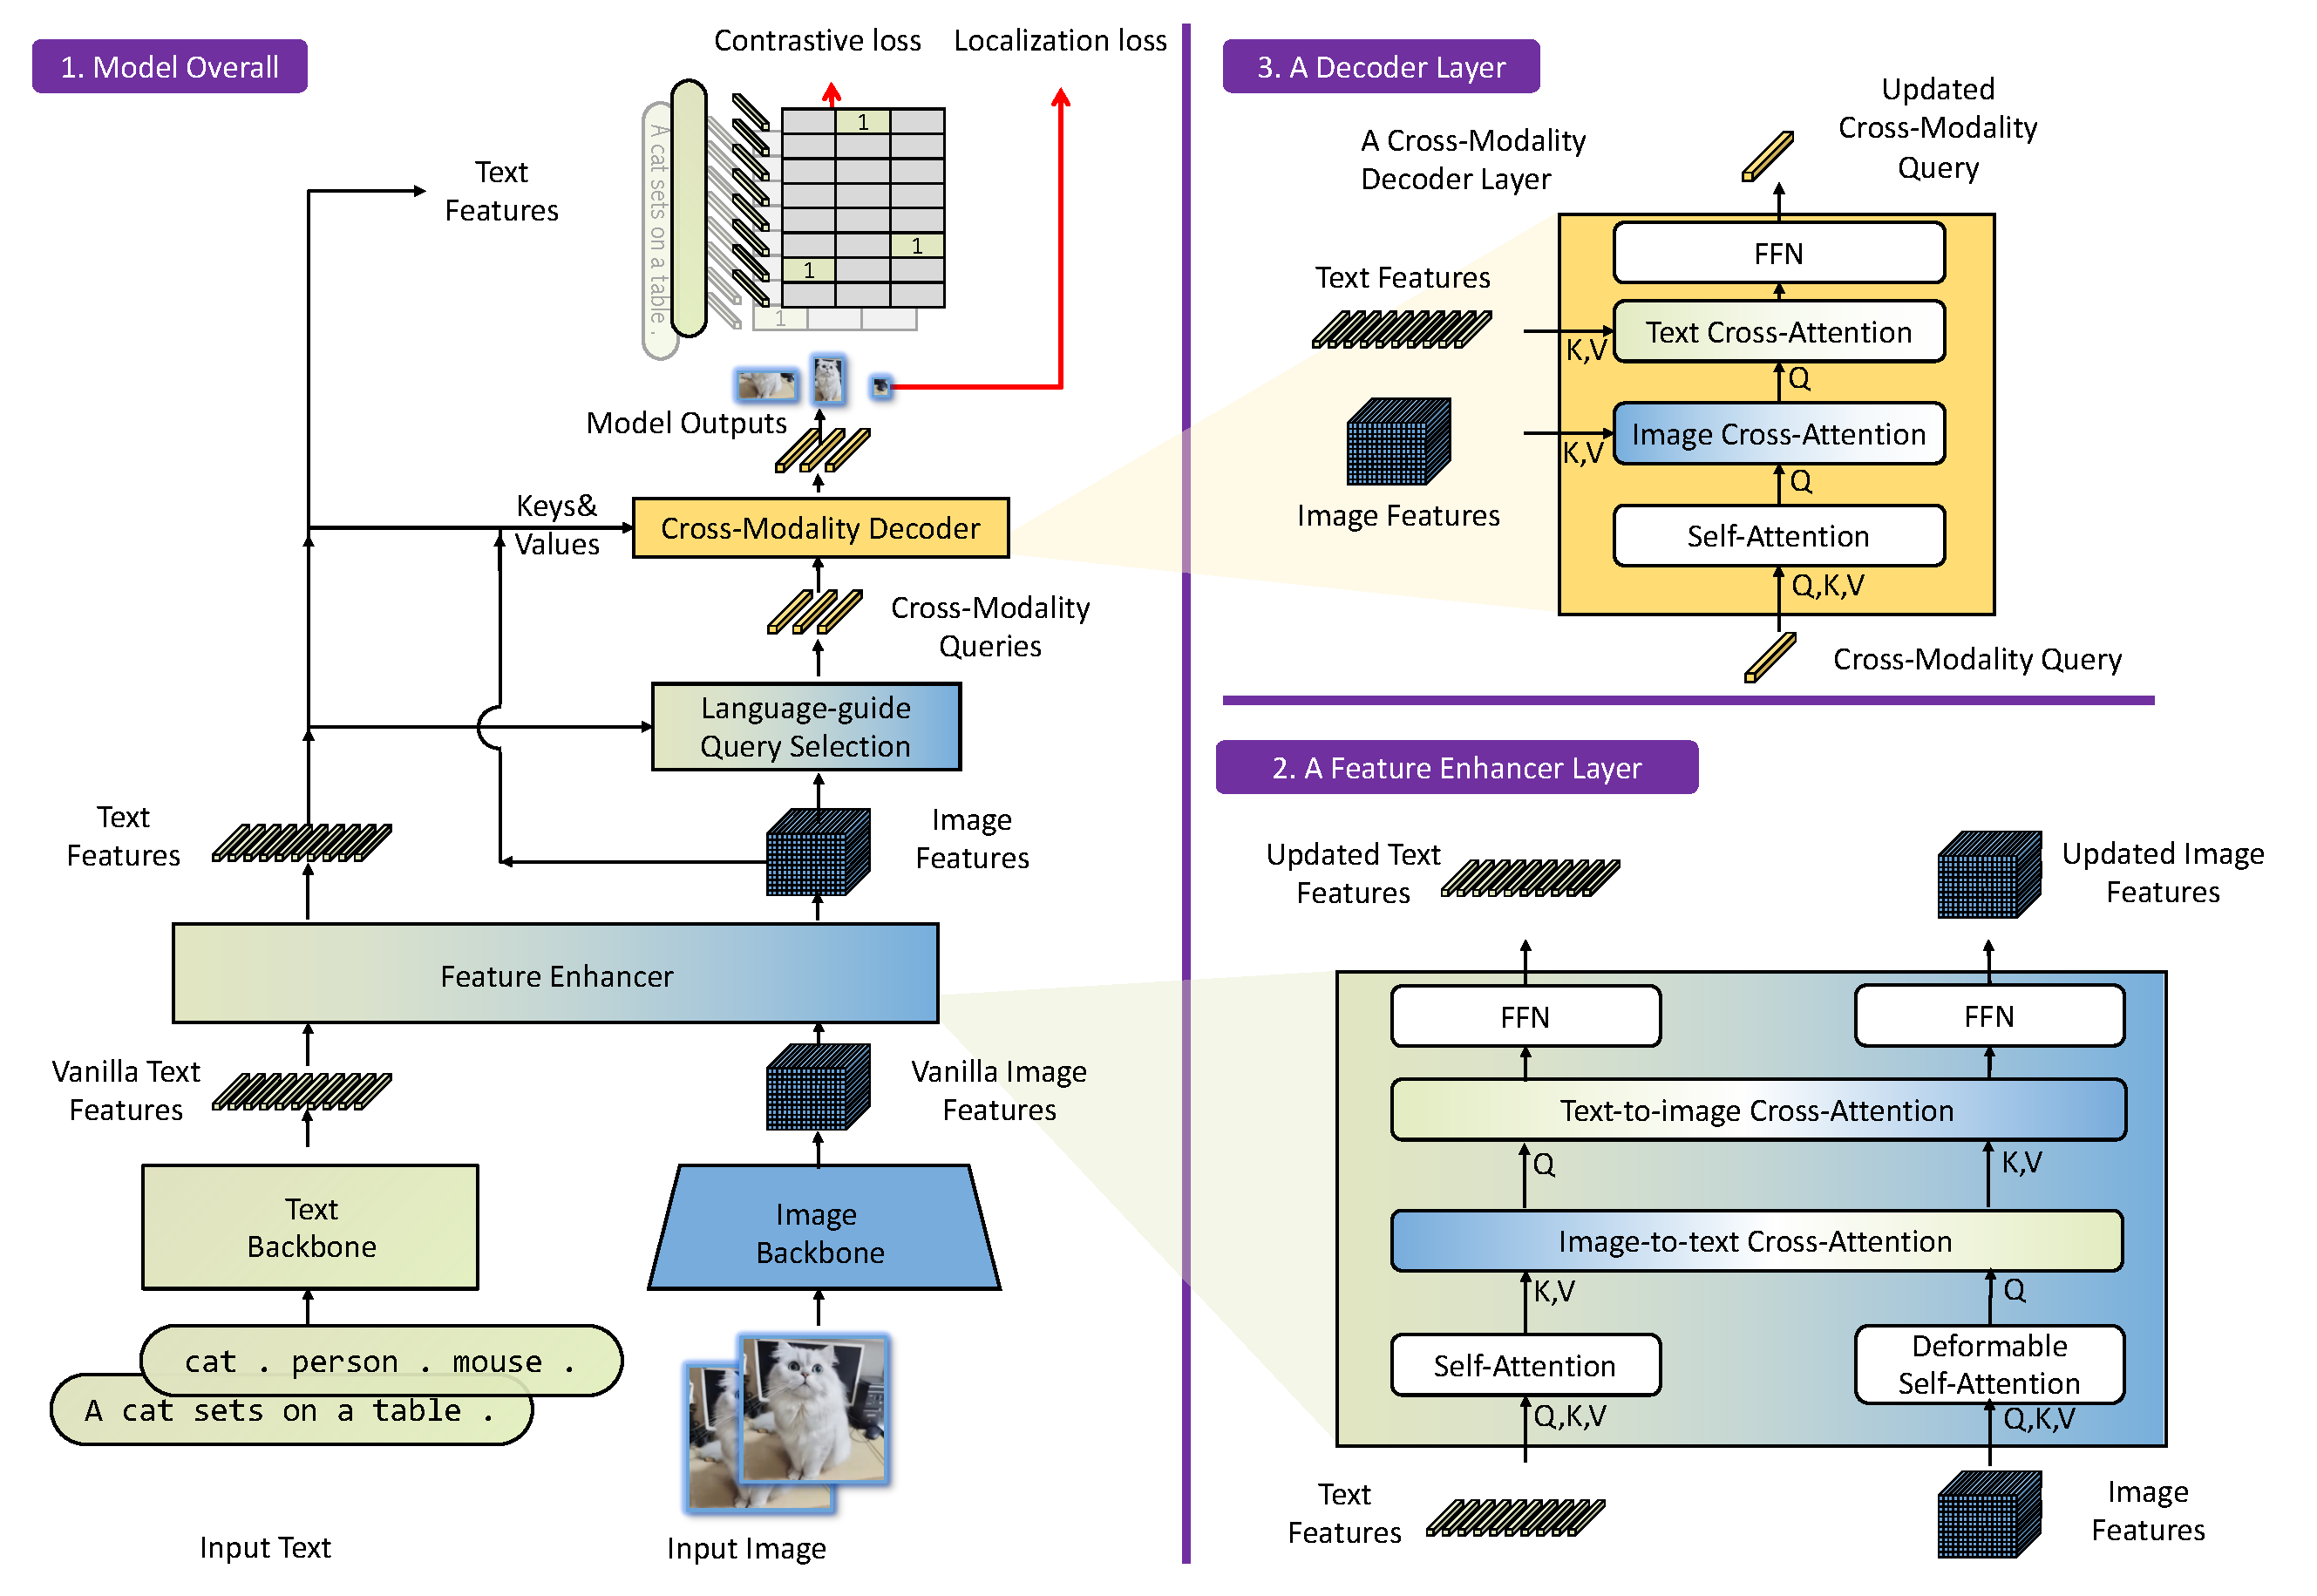
\includegraphics[width=0.98\linewidth]{Fig/fig_DINO.pdf}
    \caption{Grounding DINO as a language-guided localization module for Grounded-SAM pipelines. Text and image backbones first produce modality-specific features, a feature enhancer updates both streams, language-guided query selection initializes cross-modality queries, and the decoder predicts localized outputs under contrastive and localization losses. This architecture explains why Grounded-SAM systems often use Grounding DINO to convert text into boxes before SAM produces precise masks~\citep{liu2024groundingdino}.}
    \label{fig:promptable-groundingdino}
\end{figure}


\begin{figure*}[htbp]
    \centering
    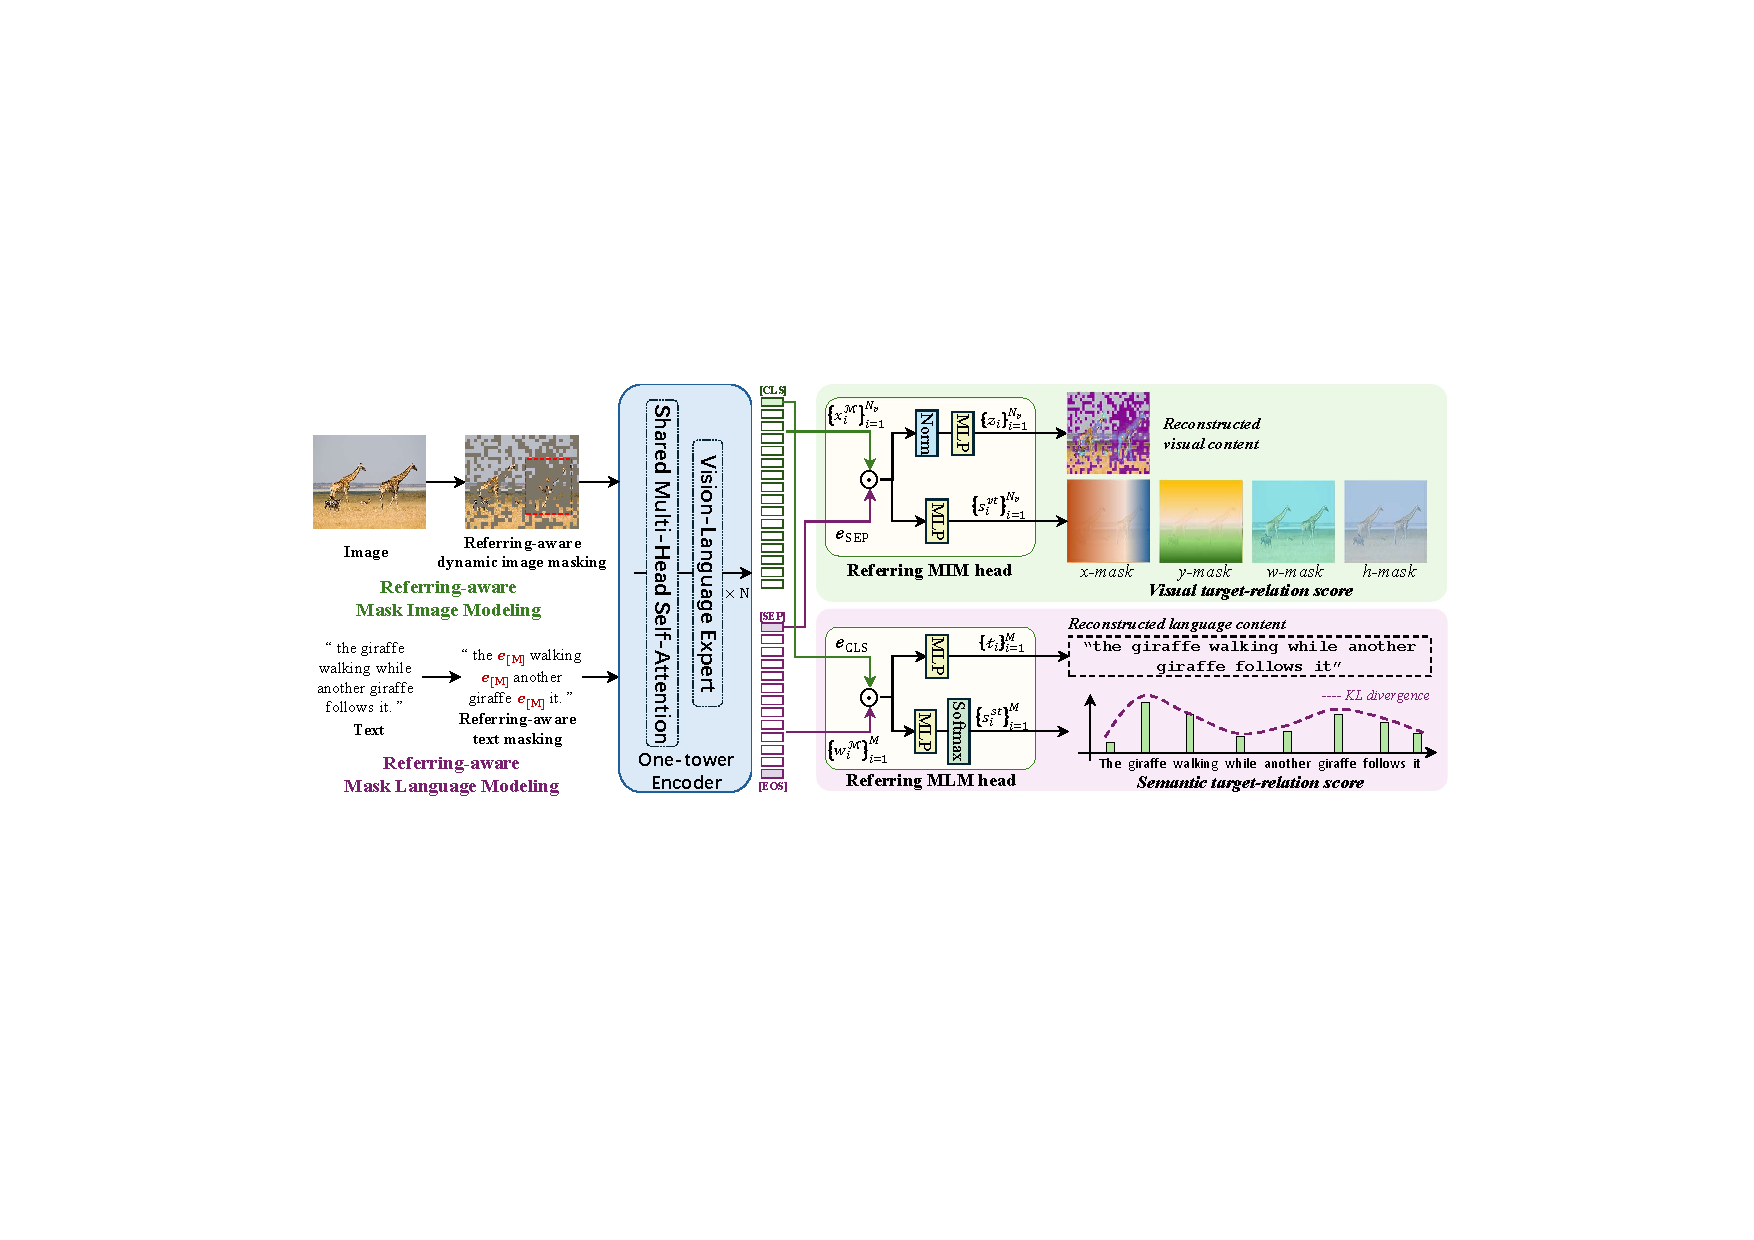
\includegraphics[width=0.98\textwidth]{Fig/fig_OneRef.pdf}
    \caption{OneRef's one-tower referring model. The image branch applies referring-aware dynamic image masking, while the text branch masks the words related to the referred target. A shared multi-head self-attention encoder feeds referring mask image modeling and referring mask language modeling heads, which reconstruct visual content and language content while scoring target-relation consistency~\citep{xiaoOnerefUnifiedOnetower2024}.}
    \label{fig:promptable-oneref}
\end{figure*}

Fig.~\ref{fig:promptable-oneref} shows a representative answer to the referring-alignment problem: both image and language are masked with awareness of the referred target, then reconstructed through a shared vision-language encoder so that visual and textual target-relation scores are learned together. More recent work broadens the referring unit from a single mask to mask groups, parts, and visual-language prompts. RAS introduces omnimodal referring expression segmentation, where a query can be text-only or text plus reference visual entities, and the output can be a group of masks rather than one region~\citep{caoReferAnySegmentation2025}. IterPrime studies zero-shot RIS and uses iterative Grad-CAM refinement with primary word emphasis to recover spatial relation sensitivity that CLIP-style masked-region ranking can miss~\citep{wangIterprimeZeroshotReferring2025}. Hybrid global-local representation similarly shows that mask-specific details and surrounding context should be combined for training-free referring segmentation~\citep{liuHybridGloballocalRepresentation2025}. These methods collectively shift the field from ``match a sentence to a mask'' toward ``ground a structured linguistic description in one or more regions.''

The advantage of region-word and mask-text grounding is that it directly attacks the language-spatial binding problem. Its limitation is that benchmark assumptions become more complex. Classic RefCOCO-style evaluation often assumes a single visible target. Generalized or open-world settings may contain multiple valid targets, no valid target, part-level targets, or ambiguous relational phrases. A fair comparison must therefore distinguish wrong target selection, incomplete masks, over-segmentation, and language misunderstanding instead of treating all errors as the same IoU drop.

\subsection{Pixel-grounded multimodal interfaces}

Grounded MLLMs turn region-word alignment into an interactive language interface. Instead of taking a category name or referring expression and returning only a mask, these systems can describe regions, accept visual prompts, output coordinates, generate grounded text, or interleave masks with dialogue. Kosmos-2 is an early example of grounding inside an MLLM: it represents object descriptions as grounded links and uses location tokens to support referring expression comprehension, phrase grounding, and referring generation~\citep{pengGroundingMultimodalLarge2024}. Ferret generalizes the input side by representing points, boxes, and free-form shapes with hybrid region features, enabling both referring and grounding at different granularities~\citep{youFerretReferGround2024}. PixelLM studies dense word grounding by allowing locations to be model inputs or outputs and regressing pixel coordinates for generated words~\citep{xuPixelalignedLanguageModel2024}.

Mask-aware instruction tuning adds pixel-level regions to the language interface. Osprey curates mask-based region-text data and uses a mask-aware visual extractor so that an MLLM can reason over precise mask regions rather than only holistic images or boxes~\citep{yuanOspreyPixelUnderstanding2024}. LLaVA-Grounding extends grounded visual chat by connecting generated responses to spatial grounding~\citep{zhangLlavagroundingGroundedVisual2024}. GLaMM goes further by generating natural-language responses interleaved with corresponding object segmentation masks, and introduces the Grounding-anything Dataset with large-scale grounded concepts and region masks~\citep{rasheedGlammPixelGrounding2024}. GroundingSuite later scales the data and evaluation side with multi-granular pixel grounding, diverse expressions, and VLM-agent annotation~\citep{huGroundingSuiteMeasuringComplex2025}.


Fig.~\ref{fig:promptable-glamm} demonstrates the interface shift from prompt-conditioned masks to grounded multimodal responses: the output is not only a segmentation mask, but a language response whose phrases can be grounded by pixel masks. These systems are important because they make segmentation part of a broader multimodal interaction loop. A user can ask about a region, request an explanation, refer to a shape, or receive grounded object mentions in a generated answer. However, this flexibility also creates new failure modes. A model may produce fluent text but attach masks to the wrong entities. It may ground only salient nouns while ignoring attributes or relations. It may return plausible masks for hallucinated objects. Therefore, pixel-grounded interfaces require joint evaluation of response correctness, grounding correctness, and mask quality, as already reflected in GroundingSuite and hallucination-oriented work reviewed later~\citep{huGroundingSuiteMeasuringComplex2025,guoSeeingBelievingRichContext2026}.

\subsection{Prompt learning and adapter-based transfer}

Prompt and adapter mechanisms provide the adaptation layer between foundation models and grounded segmentation tasks. Text prompts are easy to specify and support open-vocabulary concepts, but they can be brittle when the target concept is domain-specific, visually ambiguous, or difficult to name. Visual prompts, including points, boxes, masks, or reference examples, provide stronger spatial cues but can be sensitive to prompt placement and may not express semantic constraints. Show-or-Tell directly studies this trade-off by comparing textual and visual prompts across segmentation datasets and domains, showing that text prompts excel on common concepts while visual reference prompts can vary strongly with prompt choice~\citep{grosiShowTellBenchmark2025}.

Prompt learning methods adapt this interface rather than replacing it. Prompt-RIS uses bidirectional cross-modal prompting to produce better SAM prompts from CLIP-like alignment~\citep{cshangPromptdrivenReferringImage2024}. Visual Position Prompt adds explicit global and local spatial cues to MLLM-based visual grounding, addressing the tendency of MLLMs to privilege global semantics over precise coordinates~\citep{tangVisualPositionPrompt2026}. SAM visual projectors compress SAM-generated semantic superpixels into ``visual words'' for MLLM-based referring segmentation, reducing visual token redundancy while preserving scene-dependent geometry~\citep{yangRepurposingSAMEfficient2026}. These methods indicate that promptability is not only a user-interface property; it is also a representation and efficiency problem.

Adapter-based transfer also controls how much foundation knowledge is changed. A frozen SAM2 plus a small language adapter may preserve general promptability but struggle with specialized semantics. A tuned CLIP-SAM bridge may improve referring segmentation but risk overfitting benchmark language. A semantic projector may accelerate MLLM grounding but compress away details needed for small regions. This route should therefore be evaluated with the same discipline as open-vocabulary adaptation: report trainable parameters, prompt source, number of prompts or visual tokens, target-domain usage, and whether the evaluation includes unseen categories, unseen expressions, or unseen domains.


\begin{figure*}[htbp]
    \centering
    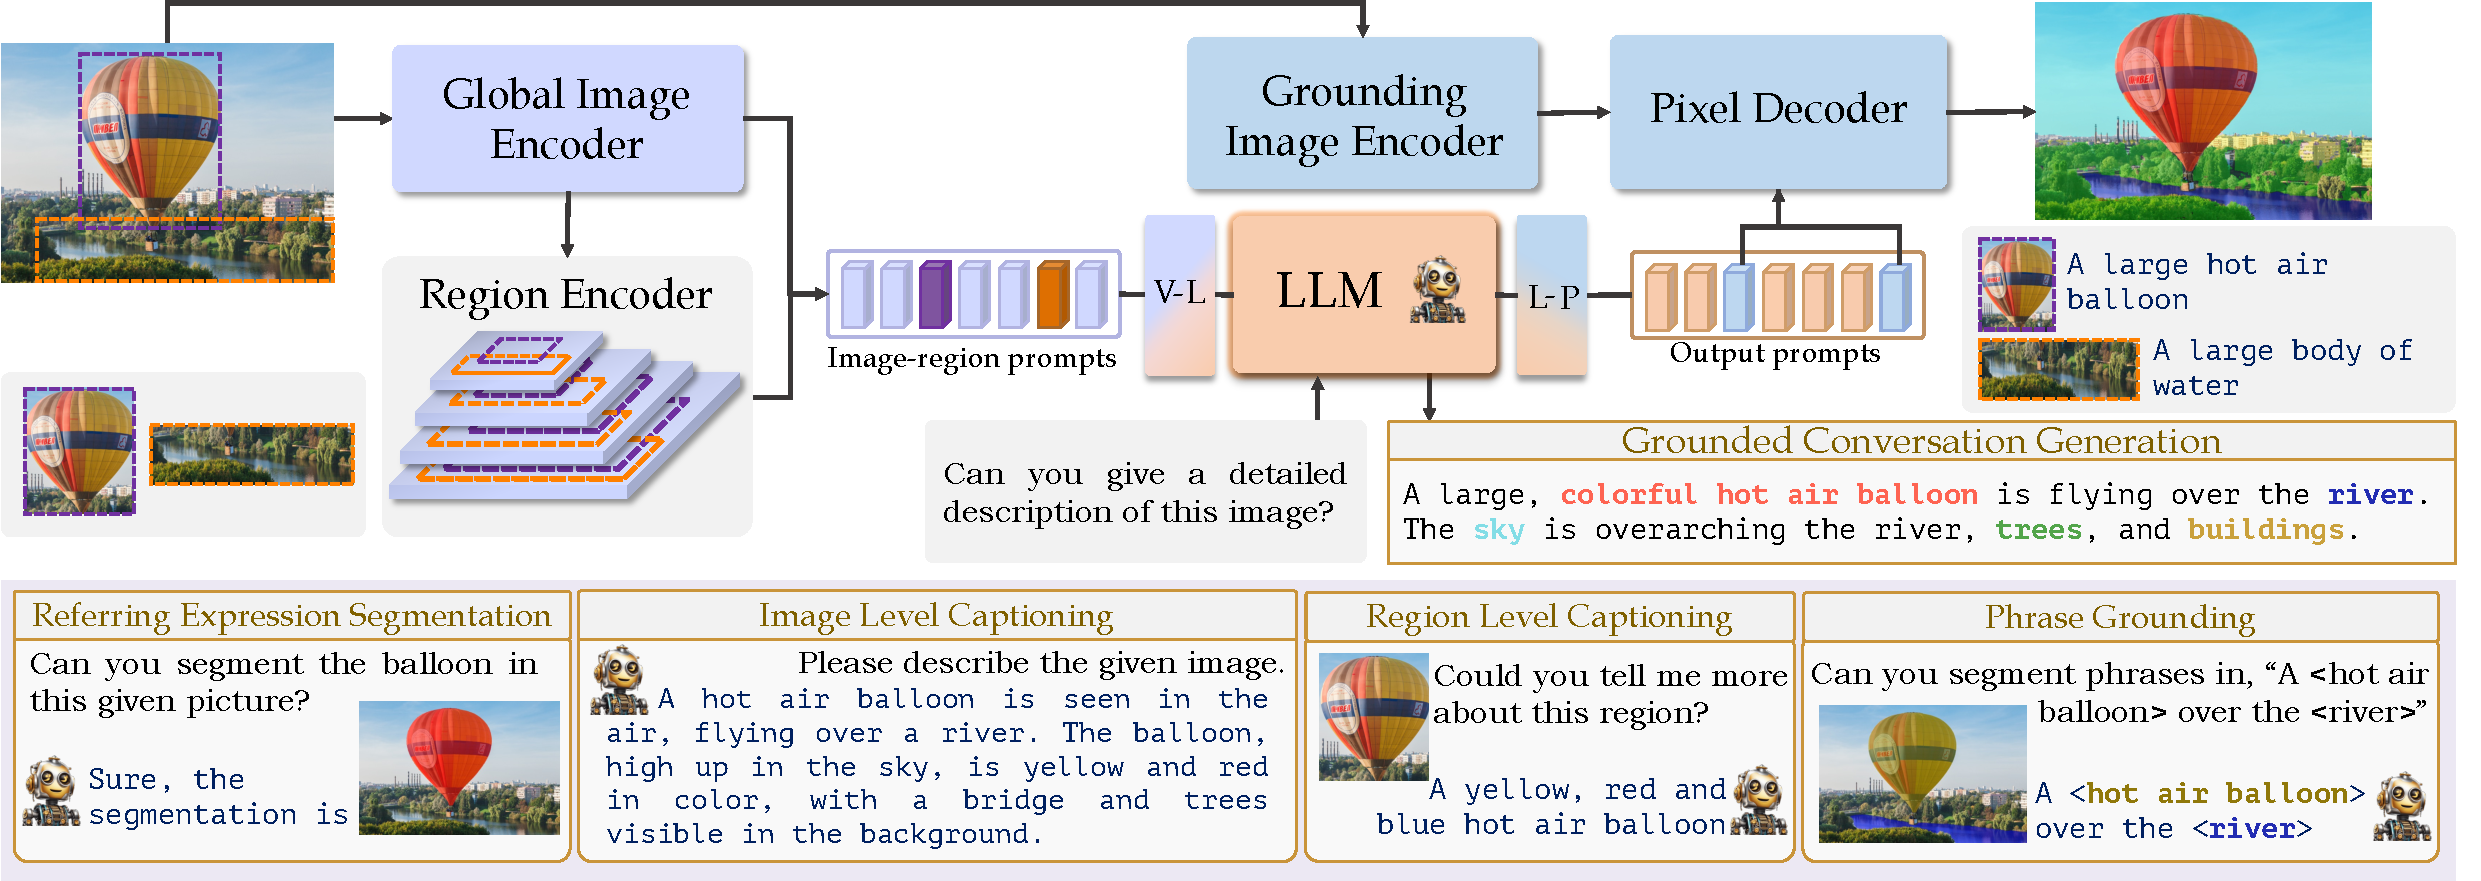
\includegraphics[width=0.98\textwidth]{Fig/fig_Glamm.pdf}
    \caption{GLaMM as a pixel-grounded multimodal conversation interface. Global image features and region features are converted into image-region prompts for the LLM, while grounding image features are passed to a pixel decoder through output prompts. The same interface supports referring expression segmentation, image-level captioning, region-level captioning, phrase grounding, and grounded conversation in which generated object mentions are linked to masks~\citep{rasheedGlammPixelGrounding2024}.}
    \label{fig:promptable-glamm}
\end{figure*}

\subsection{Summary and discussion}

Several conclusions can be drawn from this section. First, promptable segmentation supplies a powerful spatial substrate, but it does not solve semantic grounding by itself. SAM and SAM2 are strong because they make masks easy to obtain from prompts; grounded segmentation becomes necessary because users usually specify targets with language, relations, regions, or dialogue rather than with perfect points or boxes.

Second, the most common architectural pattern is decomposition. Grounded-SAM pipelines decompose text-to-mask into text-to-box and box-to-mask. Referring methods decompose expressions into words, phrases, primary nouns, relations, and mask features. Pixel-grounded MLLMs decompose interaction into generated text, spatial references, and masks. This decomposition improves modularity, but it also means that failure analysis must identify which step failed.

Third, the field is moving from single-target referring segmentation toward multi-granular grounded interaction. Mask groups, part-level references, grounded captions, region-conditioned chat, and multi-turn video grounding all require language units and mask units to be aligned at finer granularity than category names. This prepares the transition to Section~\ref{sec:reasoning-segmentation}, where the target is not always explicitly mentioned and must be inferred before it can be grounded.

Finally, promptable and grounded segmentation reveal a recurring evaluation risk. A high-quality mask can still be semantically wrong, and a semantically plausible answer can still be spatially ungrounded. Reliable comparison therefore requires reporting prompt protocols, grounding units, mask generators, language backbones, and joint text-mask metrics rather than collapsing all methods into a single segmentation score.
